\section{Training and Decision Making}%
\label{sec:tuning}

In this section, we detail the training and decision making (tuning) procedures
of the \rnn ensemble. Accordingly, we start (Section~\ref{ssec:fom}) with a
description of figures of merit that were employed.

\textcolor{red}{In short, the 2017 procedure (Section~\ref{ssec:2017}) derived the MLP ensemble\footnote{
  The ensemble is composed by one MLP model for each phase space in plan \eteta as discussed 
  in Subsection~\ref{top:nn_ensemble}. The boundaries for each one is defined by the 
  Tables~\ref{tab:comp_etabins} and~\ref{tab:comp_etbins}.} 
models with simulated data and defined the discriminant cut using
2016 collision data, targeting small signal efficiency discrepancy to triggering 
without the \rnn. The training procedure derived one ensemble (25 MLP models) for each working point (tight, medium, loose and very loose). 
The ensemble boundaries are defined by Table 4.2. 

On the other hand, the 2018 training procedure (Section~\ref{ssec:2018})
employed a single ensemble }structure for all working points and used
collision data for training, as it was the case for the derivation of offline
and final \hlt likelihood models~\cite{aaboud2019electron}.
% (since 2017~\cite{DAQ-2018-182})

\subsection{Figures of Merit}\label{ssec:fom}



The sets $\Theta_{\text{e}}$ and $\Theta_{\text{b}}$ of electrons (signal) and fake electrons (background), respectively, were selected by using the \tnp{} method and the offline selection for trigger developments (Section~\ref{ssec:dataset}). Let the existence of a model $\mathcal{C}$ representing a function $f_{\mathcal{C}} : \Theta \rightarrow \mathbb{R}$ optimized (trained) to perform the binary classification task (electron detection with background rejection). Here, $\mathbb{R}$ is the set of real numbers, as the neural network ensemble produces real numbers at the single output node for trigger decisions.  From supervised optimization, the model $\mathcal{C}$ outputs $\hat{H}:=f_{\mathcal{C}}(x)$ with target $H$ for a sample $x \in \Theta$. The operation of $\mathcal{C}$ results, respectively, in the selection of the subsets $\mathcal{O}_{\text{e}|\text{e}}$ and $\mathcal{O}_{\text{e}|\text{b}}$ from $\Theta_{\text{e}}$ and $\Theta_{\text{b}}$ as trigger candidate electrons in the \fastcalo{} processing step of the \hlt{} by defining the decision making procedure $\tau : \mathbb{R} \rightarrow \left\{\text{e},\text{b}\right\}$. As there is a single output node for each neural network in the proposed \rnn{} ensemble, $\tau$ corresponds to a mapping that is a decision threshold for selecting an electron candidate (electrons are selected when the output node is above the given threshold).  


We explicitly define some convenient figures of merit in \tablename~\ref{tab:figures_of_merit}. It is possible to tune $\mathcal{C}$ to result in a proper working point, (i.e. a targeted value of \pd{} or \pf{}) by adjusting $\tau$ (through the output decision threshold). All possible working points of $\mathcal{C}$ are defined by the Receiver Operation Characteristic (ROC) curve~\cite{van_trees_part1}, but keeping fixed the electron detection probabilities (signal efficiencies) with respect to the previous baseline trigger (cut-based). The \spindex{}~\cite{dos2006neural} is the square root of the product of the geometric and arithmetic averages of the efficiencies for the signal and background categories. It soon collapses when efficiencies on either signal or background events decrease significantly. Thus, the SP index provides a unidimensional space that allows tuning $\mathcal{C}$ for obtaining high efficiency in a balanced manner for both classes, which is given by the $\spmax{}:=\max(\spindex{})$ working point.



\begin{table}[hbt]\footnotesize
\centering
\caption{Names, symbols and definitions of the figures of merit employed. More
  than one symbol and names can be found in different fields for some figures.
  We will use the names indiscriminately throughout the text, however the
  symbols to be employed in the text are prefixed with a `$\rightarrow$' symbol.
  The unary operator $|\cdot|$ represents the cardinality of a
set.\label{tab:figures_of_merit}}
\resizebox{\textwidth}{!}{%
\begin{tabular}{cllc}
\hline
\hline
&  Symbol & Name & Definition \\
\hline
$\rightarrow$ & $\pd{}$ & Probability of detection &
\multirow{3}{*}{$\cfrac{|\mathcal{O}_{\text{e}|\text{e}}|}{|\Theta_{\text{e}}|}$}
\\
& \multirow{2}{*}{$\text{P}_{\text{e}|\text{e}}$} & Electron efficiency & \\
& & Signal Efficiency & \\
\hline
$\rightarrow$ & $\mathbf{\pf{}}$ & Probability of false alarm &
\multirow{3}{*}{$\cfrac{|\mathcal{O}_{\text{e}|\text{b}}|}{|\Theta_{\text{b}}|}$}
\\
& \multirow{2}{*}{$\text{P}_{\text{e}|\text{b}}$} & Fake rate & \\
& & Background efficiency & \\
\hline
& \spindex{} & Sum-product index & $\left(
  \left(\pd{}\cdot(1-\pf{})\right)^{\nicefrac{1}{2}} \cdot
  \left(\pd{}+(1-\pf{})\right) \cdot \nicefrac{1}{2}
  \right)^{\nicefrac{1}{2}}$ 
  \\
\hline
& MSE & Mean squared error & $\sum\limits_{x\in\Theta} \cfrac{\left(\hat{y} -
y\right)^2}{|\Theta|}$ \\
\hline
\hline
\end{tabular}
}
\end{table}





%The sets $\Theta_{\text{e}}$ and $\Theta_{\text{b}}$ of
%electrons (signal) and fake electrons (background) were selected by a reference
%method, i.e.\@ employing specialist knowledge, through requesting or vetoing some
%\tnp{} method and possibly also applying some strong classification method as
%the offline selection for trigger developments (Section~\ref{ssec:dataset}).
%Also let the existence of a model $\mathcal{C}$ representing a function
%$f_{\mathcal{C}} : \Theta \rightarrow \mathbb{R}$ optimized (trained) to
%perform the binary classification task. From supervised optimization,
%the model $\mathcal{C}$ outputs $\hat{y}:=f_{\mathcal{C}}(x)$ with target $y$ for
%a sample $x \in \Theta$. The operation of $\mathcal{C}$ results respectively in
%the selection of the subsets $\mathcal{O}_{\text{e}|\text{e}}$ and
%$\mathcal{O}_{\text{e}|\text{b}}$ from $\Theta_{\text{e}}$ and
%$\Theta_{\text{b}}$ as electrons by defining the decision making procedure
%$\tau : \mathbb{R} \rightarrow \left\{\text{e},\text{b}\right\}$. We explicitly
%define some convenient figures of merit in Table~\ref{tab:figures_of_merit}.  It
%is possible to tune $\mathcal{C}$ to result in a proper working point, (i.e.\@ a
%targeted value of \pd{} or \pf{}) by adjusting $\tau$. All possible working
%points of $\mathcal{C}$ are defined by the Receiver Operation Characteristic
%(ROC)~\cite{van_trees_part1}. The \spindex{}~\cite{dos2006neural} is the square root of the product
%of the geometric and arithmetic averages of the efficiencies for the signal and
%background categories. It soon collapses when efficiencies on either signal or
%background events decrease.  Thus, the \spindex{} index provides a
%unidimensional space, that allows to tune $\mathcal{C}$ for obtaining high
%efficiency in a balanced manner for both classes, given by the
%$\spmax{}:=\max(\spindex{})$ working point.










\subsection{2017 Procedure}\label{ssec:2017}

The training procedure and decision making processes are the same for all phase
space regions and a summary of the process is provided in
\tablename~\ref{tab:2017_ringer}. For the \rnn{}, $\mathcal{C}$ is an ensemble of
MLPs and each MLP is an expert model for a single phase space
region, containing its own topology and parameters (weights and biases).

The model parameters are optimized using events selected on simulation datasets
(Section~\ref{ssec:dataset}). The structure is a dense (fully-connected) single
hidden layer MLP, which may contain from 5 to 20 hidden units, defined through
the comparison of their efficiencies using the stratified k-fold ($\text{k}=10$)
cross-validation method~\cite{haykin_2008}. Cross-validation allows to assess the statistical fluctuations of the efficiency measurements 
at the price of increased computational cost. It is
based on repeating training and testing procedures on different
randomly chosen subsets. The stratified k-fold is
among the most common cross-validation techniques and consists of partitioning
the dataset in k disjoint subsets, each model tested with the $i$th subset and
trained with the remaining ones. The dataset stratification follows the
empirical order of the event selection, in order to allow straightforward job
parallelization, i.e.\ random permutation is not employed. The possible effect
of a temporal structure in data was neglected as 2017 training procedure
employed simulation data.

In case of similar cross-validation efficiencies when comparing standard
error confidence interval corresponding to \SI{68}{\%} for different
configurations, the choice is based on
parsimony~\cite{medeiros2001statistical}\footnote{See also discussion of the
  Minimum-description-length (MDL) principle and Occam's razor
in~\cite{haykin_2008}.} so that the structure with lower number of hidden units
is employed as higher generalization power can be expected. The activation
functions for both hidden and output neurons are the hyperbolic tangent.




\begin{table}[ht!]\footnotesize
\centering
\caption{Summary of the tuning procedure and decision making strategies employed
to obtain the \rnn for 2017 operation. See text for more
details.}\label{tab:2017_ringer}
\resizebox{\textwidth}{!}{%
\begin{tabular}{p{6cm}p{10cm}}
\hline
\hline
\hline
Criterion & Value \\
\hline
\hline
\multicolumn{2}{c}{Ensemble Composition} \\
\hline
\hline
Model & Fully connected MLP, 1 hidden-layer ($\tanh(.)$) and 1 output ($\tanh(.)$) \\
Phase space bins for Model Tuning &
See Tables~\ref{tab:comp_etabins} and \ref{tab:comp_etbins} \\
\hline
\hline
\multicolumn{2}{c}{MLP Training} \\
\hline
\hline
Core Framework & \emph{FastNet} (~\cite{tuningtools}) \\
Dataset and event selection & Simulation (Section~\ref{ssec:dataset})\\
Input Features & Concentric ring sums of energy around the particle axis  \\
Normalization & Absolute of the total ring energies (Section~\ref{top:pp}) \\
Cost-function for tuning & MSE \\
Back-propagation method & RPROP (default parameters, except $\eta^+=1.1$) \\
Targets (Electron/Background) & +1/-1 \\
Batch size & Number of observations in the smaller class \\
Maximum number of training epochs & $\infty$ \\

Over-training evaluation & Multi-stop (see text) using
50 epochs stop criterion \\

Working point reference & Baseline chain efficiencies at \hltcalo \\

Evaluated structures & Number of hidden units ranging from 5 to 20 units \\

Initializations & 100 (Nguyen-Widrow method) \\

Cross-validation method & Stratified k-fold ($k=10$, validation set used for
both testing and early stop computation) \\

Cross-validation subset retrieval method & Split data uniformly into k subsets,
random permutation not applied. Remaining samples are put one by one into the
first subsets \\
ROC extraction method & 1,000 linearly spaced points between model targets \\
\hline
\hline
\multicolumn{2}{c}{Training Evaluation and Operating Model Selection } \\
\hline
\hline

Working Point & ROC point closest to signal efficiency reference and \spmax{}
value \\

Best Initialization Choice & Lowest fake rate (validation set) when operating in
a region of up to $\epsilon=0,2~\%$ of the reference signal efficiency \\

Model Topology Selection & Graphical analysis using box plots \\

Operating Model Choice & Lowest fake rate (using full stats.) when operating in
a region of up to $\epsilon=0,2~\%$ of the reference signal efficiency \\

Operation Extrapolation & Yes, eventual observations outside model phase
space regions use the nearest expert model (in lowest Euclidean
distance in $\et\times\eta$ axis) \\

\hline
\hline
\multicolumn{2}{c}{Decision Making} \\
\hline
\hline

Pile-up Efficiency Correction & Compute straight-line balancing efficiency within
$\avgmu=[0,20,40]$ avg.\@ collisions \\
Dataset and event selection & 2016 $13\;\text{TeV}$ p-p collision data
(GRL: v88), except for reprocessing reference run \\
Decision Making Strategy & Linear fit to the network output without applying the
transfer function w.r.t. $\avgmu$ up to 40$\;$avg.\@ collisions.
When $\avgmu>40$, set $\avgmu = 40$ (2016 upper bound) \\
%Cross-Validation Method & None \\

Phase space bins for Linear Fit & See
Tables~\ref{tab:comp_etabins} and~\ref{tab:comp_etbins} \\
Target Working Point & Keep HLT signal efficiency of the proposed chain as near
as possible from the respective baseline chain \\
\hline
\hline
\hline
\end{tabular}
}
\end{table}





For each cross-validation sort and working point, 100 networks, initiated
as from~\cite{initnw}, are optimized by back-propagating MSE through the RPROP
algorithm~\cite{rprop} with all parameters set to default, except for
$\eta^+=1.1$ (default is 1.2). This particular
parameter regards the multiplication factor of the weight update rate when
gradient direction remains the same as of the previous iteration. It was
observed during Run~1 that this modification improved convergence speed. RPROP
is an adaptive gradient descendent technique that is resilient to the size of
the derivatives. This repeated model initialization aims at
avoiding poor sub-optimal solutions due to usage of gradient-based algorithms as
RPROP in optimisation problems involving non-convex and complex function.
For each training procedure, only three models out of the 100 are retained: two
for retrieving the best efficiency when fixing the \pd{} or \pf{} to the
baseline \fastcalo{} efficiency and another resulting in the \spmax{} value.
Early stopping~\cite{haykin_2008} is employed to avoid model over-training. The
selection of the optimal iteration and operating model is based on an heuristic
approach (multi-stop).


Computational resources from the WLCG and \emph{Lobo Carneiro}
super-cluster~\cite{lobo_carneiro} were used to tune 1.3~M shallow-learning
neural networks, which resulted in an ensemble of \SI{20}{MLPs} (five in \et{}
$\times$ four in \abseta{})  for each one of the four working points used by
electron chains in the HLT (see Section~\ref{ssec:egamma_trigger}).\@ Except 
for few exceptions, the models in the ensemble employed 5 neurons in the 
hidden layer.  Thus, for 2017 operation, 
\rnn{} operation did not result on
successive contained sets for more stringent working points, i.e. an electron
candidate accepted by \medium{} is not necessarily also accepted by \loose{}
working point. %To the best of our knowledge, this does not impact the \hlt{}
%given that triggers are employed in parallel both for operation and analysis.
%Thus, eventual disagreements between their selections are irrelevant.


After the training stage, the decision is taken by applying a threshold in the
one-dimensional output node of each expert MLP.\@ 
Inspired by the HLT likelihood algorithm, the threshold applied for
\rnn is also computed as a linear function of \avgmu{}.
However, when employing the standard NN parametrisation, a non-linear
behavior was observed near the asymptote of the output activation 
function (See Figure~\ref{fig:nn_correction_with_tansig}) which occured
for the medium and tight operation points. Heuristically, it was 
observed that this behaviour can be avoid when replacing the output
activation by a linear function (Figure~\ref{fig:nn_correction_without_tansig})
for operation (after the training stage is completed).
This strategy sufficed to achieve linear
behavior of the targeted signal efficiency with respect to the online pile-up
estimator. Except for the end-cap region during 2017, the boundaries for
defining discriminant requirement parameters were the same as those employed in
the \rnn ensemble (Section~\ref{top:nn_ensemble}). The interpolation in
\et{} employed in the likelihood as a smoothening
strategy~\cite{aaboud2019electron} was not used
(Section~\ref{ssec:egamma_trigger}).  Tables~\ref{tab:comp_etabins}
and~\ref{tab:comp_etbins} show the boundaries in the \eteta{} axis used for
Run~2 operation.



\begin{figure}[h!tb]
  \begin{center}
  %\hspace{0.01\textwidth}
  \begin{subfigure}[c]{.48\textwidth}
  \centering
  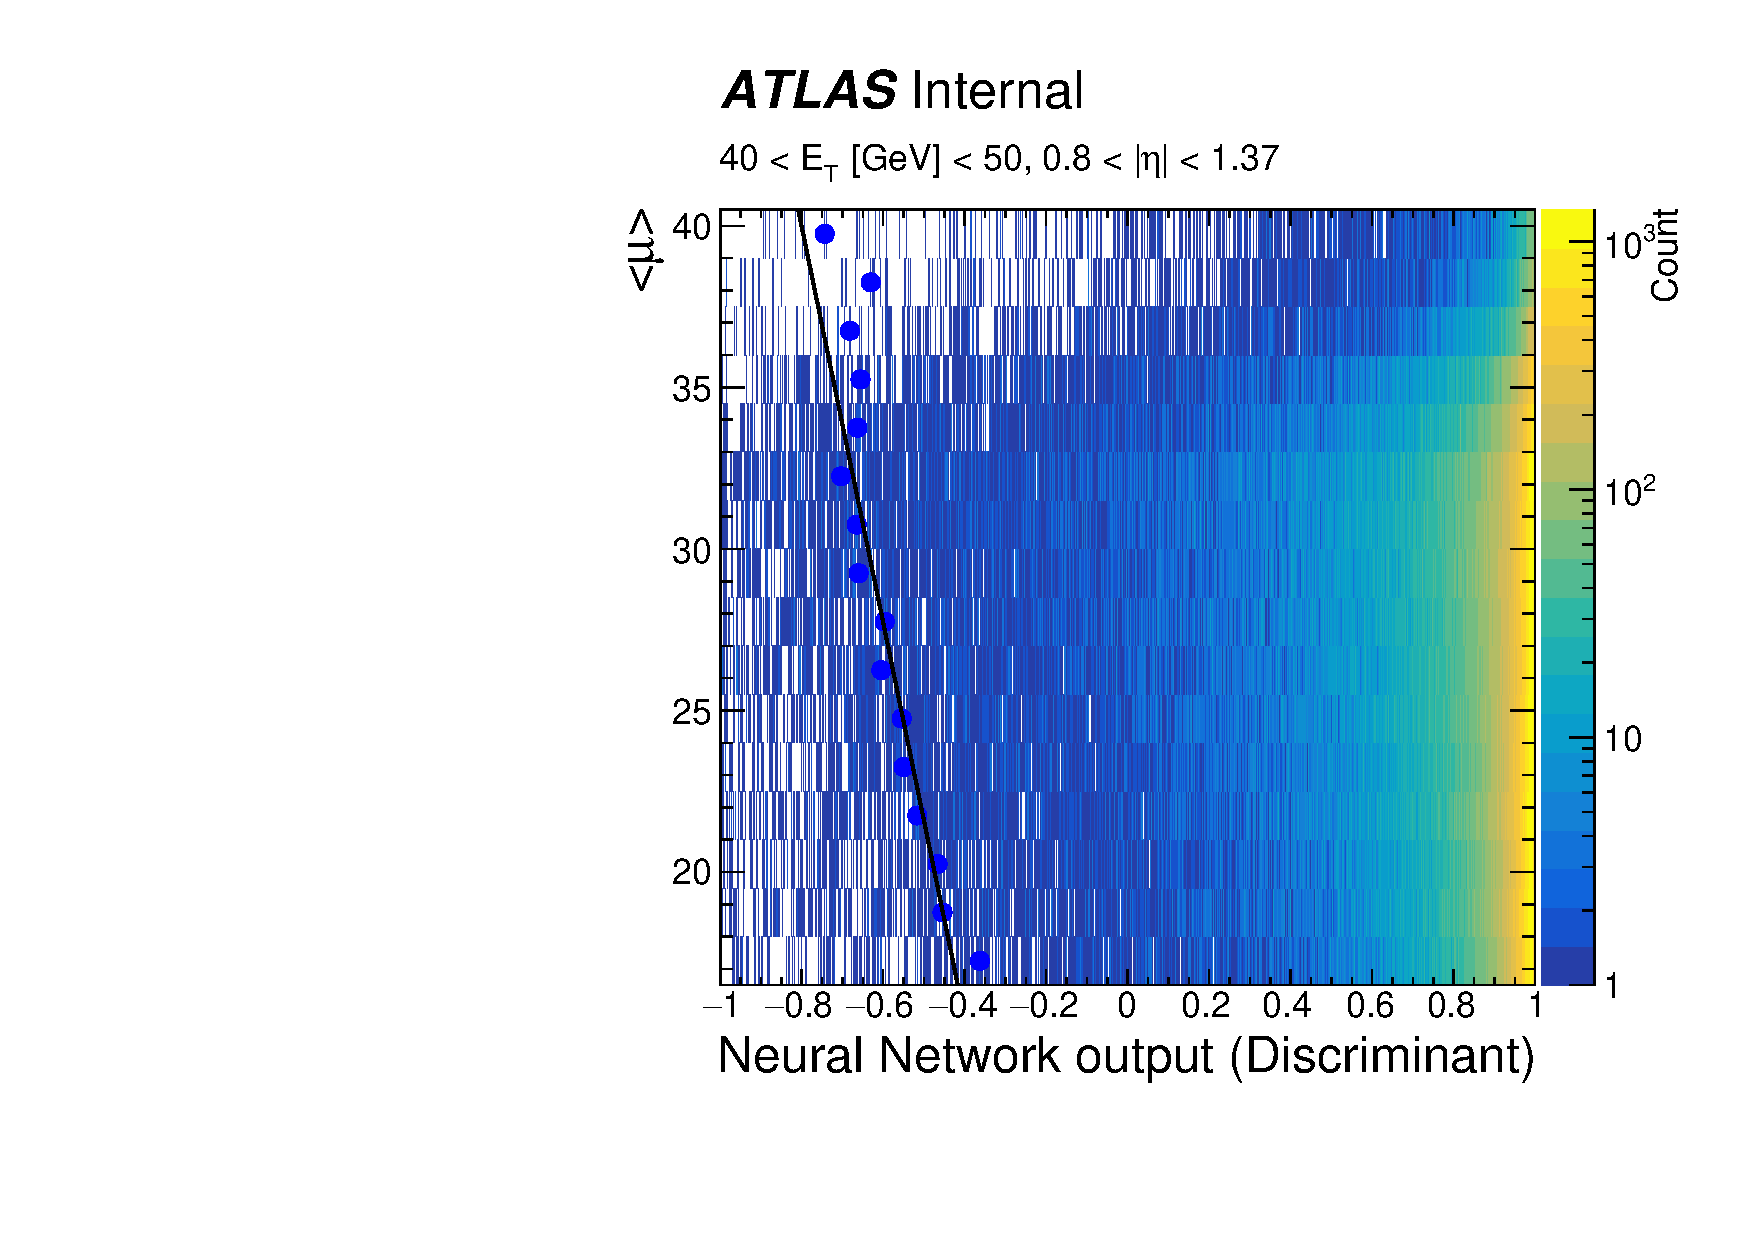
\includegraphics[width=\textwidth]{sections/tuning_strategy/figures/hist2D_signal_pileupCorrection_with_tansig_et3_eta1.pdf}
  \caption{Neural output with hyperbolic tangent w.r.t pileup.}
  \label{fig:nn_correction_with_tansig}
  \end{subfigure}
  \hfill
  \begin{subfigure}[c]{.48\textwidth}
  \centering
  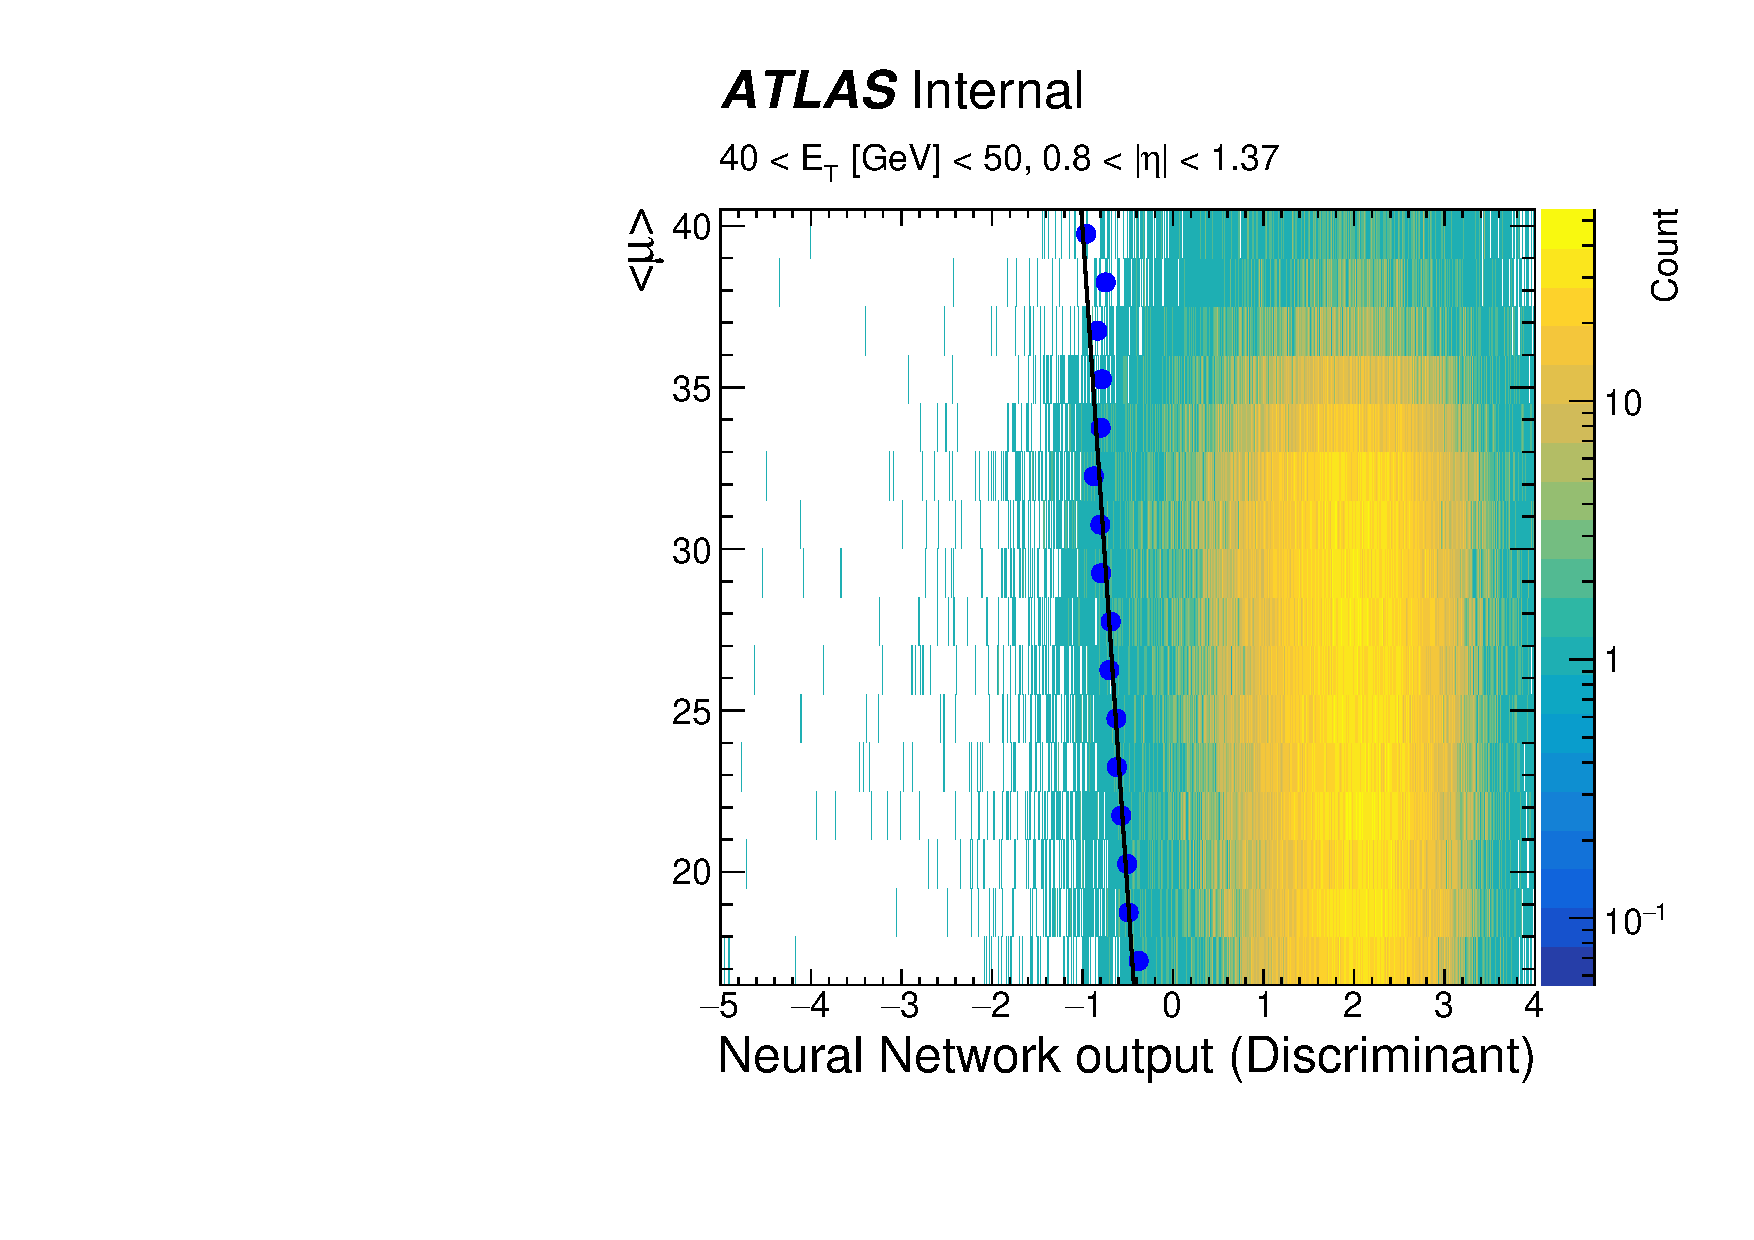
\includegraphics[width=\textwidth]{sections/tuning_strategy/figures/hist2D_signal_pileupCorrection_without_tansig_et3_eta1.pdf}
  \caption{Neural output with linear activation w.r.t pileup.}
  \label{fig:nn_correction_without_tansig}
  \end{subfigure}
  %\hfill
  \caption{
    \rnn output as a function of \avgmu{} for $Z\rightarrow ee$ probes in 
    2016 collision data.
    The computed threshold per \avgmu{} unit for achieving the target 
    efficiency is shown in blue full circle. The black line is a linear fit of the thresholds.
    The output space is computed using the traind model without modifications 
    in (a), while in (b) the output activation is replaced by the identity.
    The electron probes are selected using the training criteria.
  }%
  \end{center}
  \end{figure}





\begin{table*}[htb]
\caption{Boundaries in absolute electron pseudorapidity used to define the bins
  of the ensemble. The term `MLP' refers to the boundaries for the operation of
  the \rnn{} specialist network and with the `discriminant' term we define the
  boundaries for defining the thresholds for each requirement. Here, \emph{both}
refers to the computation of either the model parameters or the discriminant
respecting the same boundaries.}%
\label{tab:comp_etabins}
\begin{center}
\begin{tabular}{lcccccc}
\hline
\multicolumn{7}{c}{2017 \rnn  bin boundaries in \abseta}\\
\hline
MLP & 0.0 & 0.8& 1.37& 1.54& & 2.5 \\
Discriminant & 0.0& 0.8& 1.37& 1.54& 2.37 & 2.5 \\
\hline
\multicolumn{7}{c}{2018 \rnn  bin boundaries in \abseta}\\
\hline
Both & 0.0 & 0.8& 1.37& 1.52& 2.37 & 2.47 \\
\hline
\end{tabular}
\end{center}
\end{table*}






\begin{table*}[htb]
\caption{Boundaries in electron transverse energy defining the specialist
  network and discriminant threshold values to be employed by the \rnn{}
  algorithm.
}%
\label{tab:comp_etbins}
\begin{center}
\begin{tabular}{cccccc}
\hline
\multicolumn{6}{c}{2017 and 2018 \rnn bin boundaries in \Et [\GeV]}\\
\hline
15& 20& 30& 40& 50 & $\infty$ \\
\hline
\end{tabular}
\end{center}
\end{table*}






% TODO A plot showing the particular impact in the 2.37 region
% TODO Cross-validation: error bars
% TODO MLP training example
\begin{figure}[h!t]
\centering
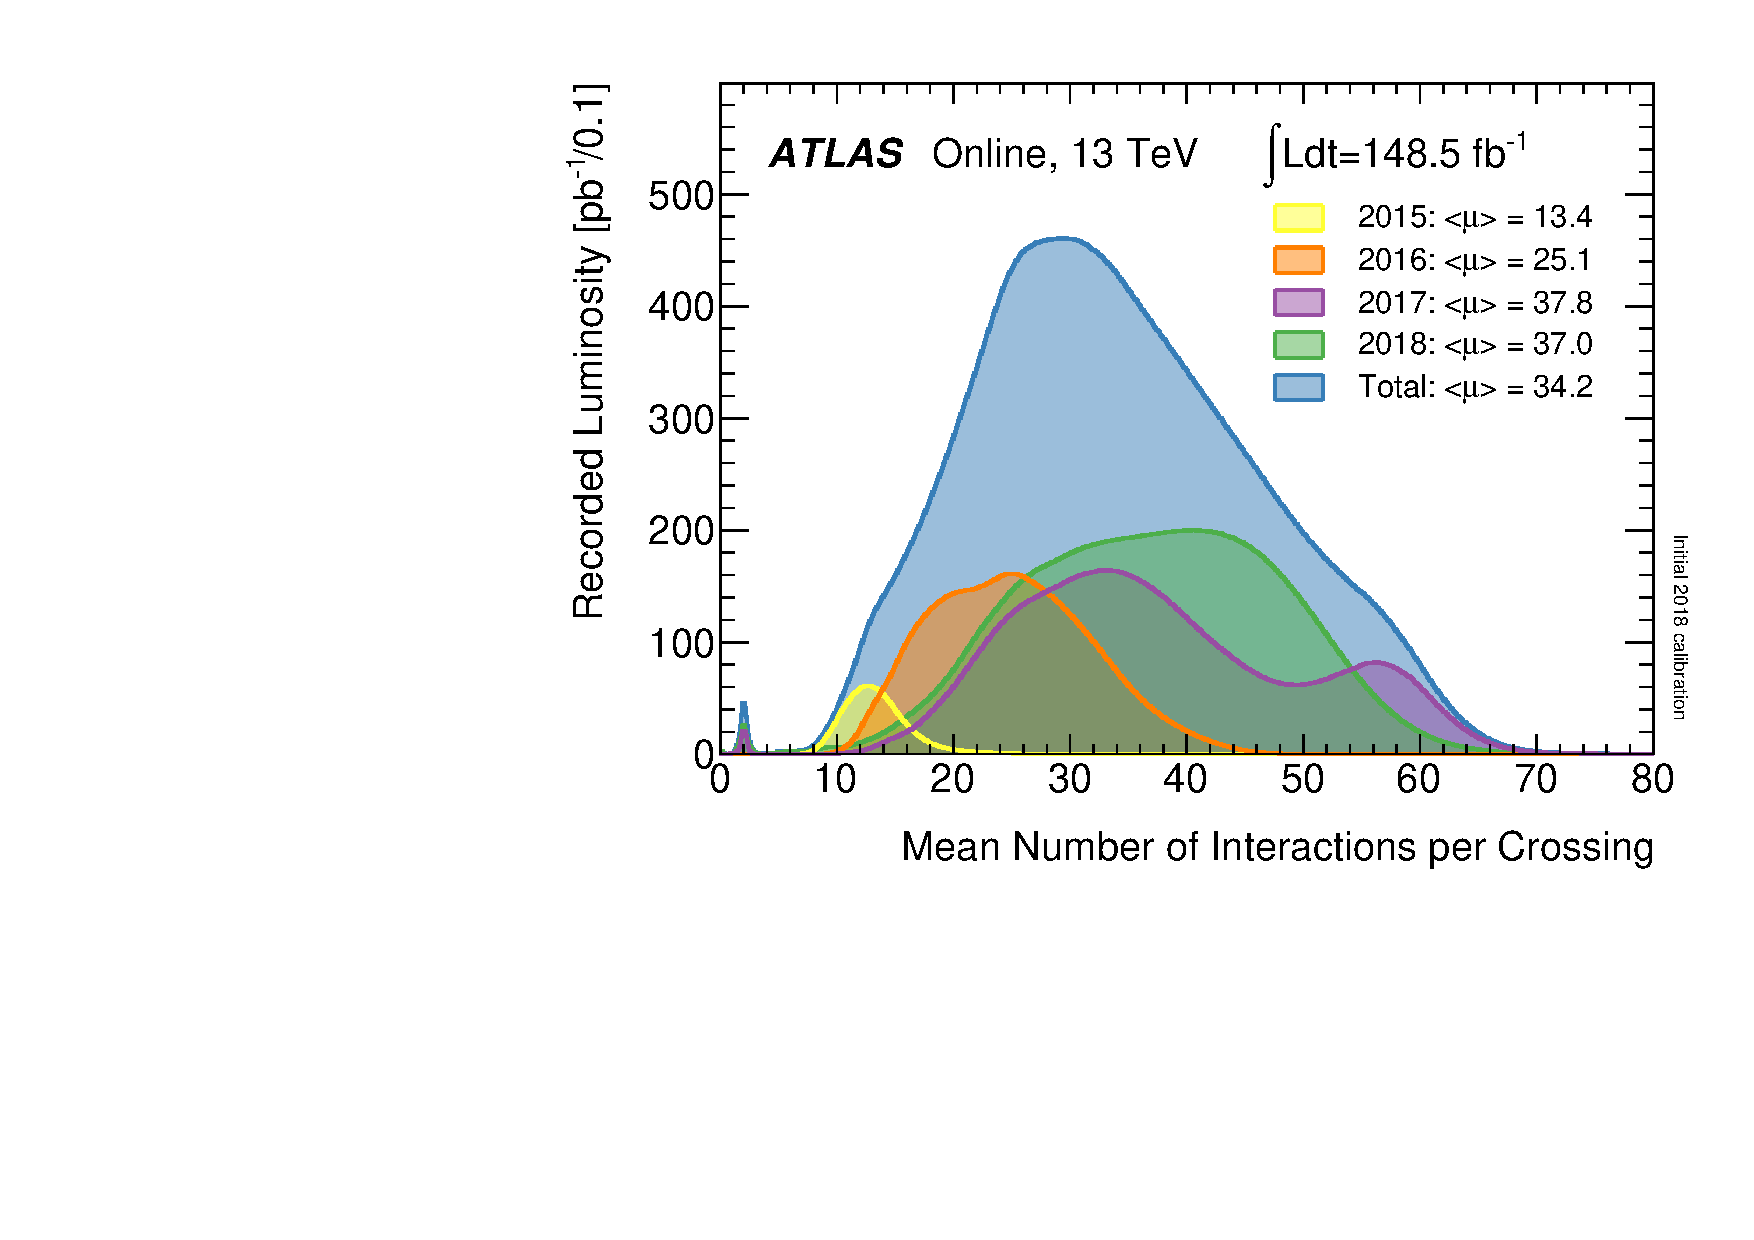
\includegraphics[width=0.6\textwidth]{sections/tuning_strategy/figures/mu_2015_2018.pdf}
\caption{\label{fig:mu_2015_2018}
Luminosity-weighted distribution of the mean number of interactions per crossing
for the Run~2 pp collision data at 13 TeV centre-of-mass
energy.~\cite{atlas_lumi_run2_results}}
\end{figure}


The linear correction applied during 2017 is upper-bounded by $\avgmu=40$
collisions, a quantile encompassing a large fraction of 2016 data
(Figure~\ref{fig:mu_2015_2018}). The objective was to avoid extrapolation to a
regime not previously evaluated, which could lead to unexpected growth in the
background rate and, thus, to data-taking issues due to the large CPU demand
from the electron triggers.

% (decision taking)
To account for Monte Carlo data mis-modeling, the parameters of the linear threshold
correction were derived using 2016 collision data. Furthermore, it was observed
that the rings in the region $2.37<\abseta<2.47$ had particular profiles due to
the lack of strip cells in this region (\tablename~\ref{tab:granularity}). It
drastically affected the ring profiles in this region which resulted in a shift
of the signal discriminant towards the direction of the background target and
demanded a specific discriminant requirement in order to keep signal
efficiencies near triggers without \rnn{}.

\FloatBarrier
\subsection{2018 Procedure}\label{ssec:2018}

Most of procedure was kept unchanged for 2018, with modifications shown in
Table~\ref{tab:2018_ringer}. In opposition to 2017, the developments for 2018
could benefit from collision data representing similar conditions to data taking.
Specifically, the 2017 LHC limitation was
fixed and the experiments expected to benefit from a proper filling scheme
resulting in lower pile-up conditions for the same luminosity. The major
alteration in 2018 tunes was the derivation of the \rnn{} ensemble with
collision data based on \Zee{} \tnp{} event selection, in order to avoid the
Monte Carlo data mis-modeling.

We also simplified the training strategy by abandoning the selection of three
models for each training and keeping only the \spmax{} model as the previous approach was more complex without a clear
payoff in trigger efficiency.
Likewise, we tuned MLPs with 5 to 10 units in the (single) hidden layer, as most models did not require
more than 10 units in 2017. With a larger time span for entering operation, we
added MLPs specialized in the region where we detected a change in the ring
profiles before 2017 operation ($2.37<\abseta<2.47$), resulting in the operation of
\SI{25}{MLPs}. The fit method was updated to match the new likelihood strategy with a
goodness-of-fit minimization. The correction limit was set to
$\avgmu{}=100$~collisions or, in other words, removed for 2018 operation, given
that the data-taking conditions did not extrapolate this value. By assuming a
linear efficiency extrapolation,%\footnote{It is worth noticing that the linear
%fit is reasonably good for the Run~2 conditions.}
we observed that most phase space regions did not reach background efficiencies
larger than \SI{15}{\%} before arriving at $\avgmu=100$~collisions, while same
signal efficiencies were maintained.

% NOTE TriggerEgammaMeeting_20180213

% NOTE TriggerEgammaMeeting_20180213

\begin{table}[ht!]\footnotesize
\centering
\caption{Changes in the derivation of the 2018 \rnn operation models with
respect to 2017 models. See text for more details.}\label{tab:2018_ringer}
\resizebox{\textwidth}{!}{%
\begin{tabular}{p{6cm}p{10cm}}
\hline
\hline
\hline
Criterion & Value \\
\hline
\hline
\multicolumn{2}{c}{Ensemble Composition} \\
\hline
\hline
Phase space bins for Model Tuning &
Added one new boundary for the tunes in \eta, see Table~\ref{tab:ensemble_regions} \\
\\
\hline
\hline
\multicolumn{2}{c}{MLP Training} \\
\hline
\hline

Dataset and event selection & 2017 $13$ TeV $p-p$ collision data (Section~\ref{ssec:dataset})
\\ 
Over-training evaluation & Stop when fail to improve \spmax for 50 epochs
(compute ROC at each epoch) \\

Evaluated topologies & Hidden layer with number of neurons ranging from 5 to 10
units \\

\hline
\hline
\multicolumn{2}{c}{Training Evaluation and Selection of the Operating Model} \\
\hline
\hline

\multicolumn{2}{c}{All criteria with same configuration} \\

\hline
\hline
\multicolumn{2}{c}{Decision Making} \\
\hline
\hline

Fit Method & Linear fit method
$\chi^2=\frac{{(y-f(x))}^2}{e_y^2+{(0,5{(e_{xl}+e_{xh})}f\prime(x))}^2}$ 
\textcolor{red}{where $f(x)$ is the function to be fitted, in this case an affine function; and $y$ is the lower (upper) error of the ordinates if $f(x)$ is below (above) $y$, and $e_{xl}$ ($e_{xh}$) is the lower (upper) error on the abscissas.} \\
Dataset and event selection & 2017 $13\;\text{TeV}$ p-p collision data (GRL:
v97), except for reprocessing reference run \\

Decision Making Strategy & Linear fit of the network \textcolor{red}{output by replacing the transfer function} w.r.t. $\avgmu$ up to 100$\;$avg.\@ collisions.
When $\avgmu >100$, set $\avgmu = 100$ \\

\hline
\hline
\hline
\end{tabular}
}
\end{table}




